% https://www.latex4technics.com/?note=m4u
% https://tex.stackexchange.com/q/210367/173708

 \documentclass[tikz]{standalone}
\begin{document}

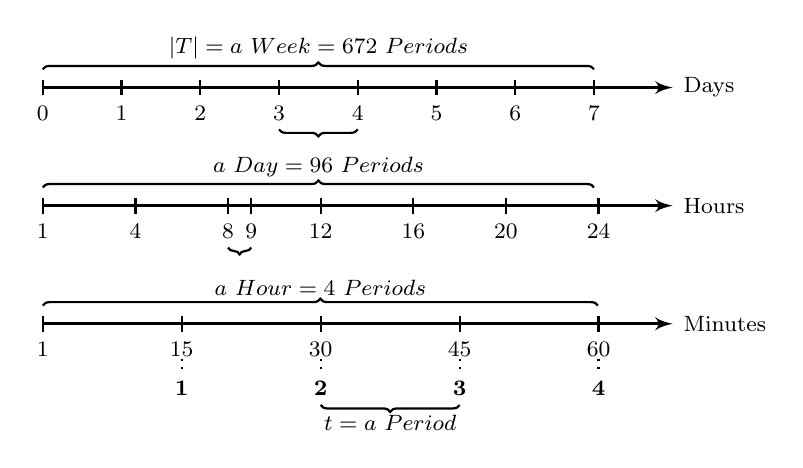
\begin{tikzpicture}[y=1cm, x=1cm, thick, font=\footnotesize]    
\usetikzlibrary{arrows,decorations.pathreplacing}

\tikzset{
   brace_top/.style={
     decoration={brace},
     decorate
   },
   brace_bottom/.style={
     decoration={brace, mirror},
     decorate
   }
}

% time line week
\draw[line width=1.2pt, ->, >=latex'](0,0) -- coordinate (x axis) (8,0) node[right] {Days}; 
\foreach \x in {0,...,7} \draw (\x,0.1) -- (\x,-0.1) node[below] {\x};

% top brace
\node (start_week) at (0,0.1) {};
\node (end_week) at (7,0.1) {};
\draw [brace_top] (start_week.north) -- node [above, pos=0.5] {$|T| =a~Week = 672~Periods$} (end_week.north);

% low brace
\node (start_day_u) at (3,-0.4) {};
\node (end_day_u) at (4,-0.4) {};
\draw [brace_bottom] (start_day_u.south) -- node [below, pos=0.5] {} (end_day_u.south);

% time line day
\draw[line width=1.2pt, ->, >=latex'](0,-1.5) -- coordinate (x axis) (8,-1.5) node[right] {Hours}; 
\draw (0,-1.4) -- (0,-1.6) node[below] {1};
\foreach \x in {4,8,12,16,20,24} \draw (\x/3.4,-1.4) -- (\x/3.4,-1.6) node[below] {\x};
\draw (9/3.4,-1.4) -- (9/3.4,-1.6) node[below] {9};

% top brace
\node (start_day) at (0,-1.4) {};
\node (end_day) at (7,-1.4) {};
\draw [brace_top] (start_day.north) -- node [above, pos=0.5] {$ a~Day = 96~Periods$} (end_day.north);

% low brace
\node (start_hour_u) at (8/3.4,-1.9) {};
\node (end_hour_u) at (9/3.4,-1.9) {};
\draw [brace_bottom] (start_hour_u.south) -- node [below, pos=0.5] {} (end_hour_u.south);

% time line hour
\draw[line width=1.2pt, ->, >=latex'](0,-3.0) -- coordinate (x axis) (8,-3.0) node[right] {Minutes}; 
\draw (0,-2.9) -- (0,-3.1) node[below] {1};
\foreach \x in {15,30,45,60} \draw (\x/8.5,-2.9) -- (\x/8.5,-3.1) node[below] {\x};

% top brace
\node (start_hour) at (0,-2.9) {};
\node (end_hour) at (7.05,-2.9) {};
\draw [brace_top] (start_hour.north) -- node [above, pos=0.5] {$ a~Hour = 4~Periods$} (end_hour.north);

% time line period
\foreach \x in {1,...,4} \draw[dotted] (15*\x/8.5,-3.45) -- (15*\x/8.5,-3.6) node[below] {\textbf{\x}};

% low brace period
\node (start_period) at (30/8.5,-3.9) {};
\node (end_period) at (45/8.5,-3.9) {};
\draw [brace_bottom] (start_period.south) -- node [below, pos=0.5] {$t=a~Period$} (end_period.south);

\end{tikzpicture}
\end{document}
